% Created 2024-03-14 Thu 12:51
% Intended LaTeX compiler: pdflatex
\documentclass[11pt]{article}
\usepackage{amsmath}
\usepackage[utf8]{inputenc}
\usepackage[T1]{fontenc}
\usepackage{graphicx}
\usepackage{longtable}
\usepackage{wrapfig}
\usepackage{rotating}
\usepackage[normalem]{ulem}
\usepackage{amsmath}
\usepackage{amssymb}
\usepackage{capt-of}
\usepackage{hyperref}
\usepackage{listings}
\usepackage[margin=2.5cm,headheight=66pt]{geometry}
\usepackage{enumitem}
\usepackage{fancyvrb}
\usepackage[magyar, american]{babel}
\usepackage[utf8]{inputenc}
\usepackage[TS1,T1]{fontenc}
\hypersetup{hidelinks=true}
\date{}
\title{Parallel self-adjusting packet classification: Initial results}
\hypersetup{
 pdfauthor={retvari},
 pdftitle={Parallel self-adjusting packet classification: Initial results},
 pdfkeywords={},
 pdfsubject={},
 pdfcreator={Emacs 29.1 (Org mode 9.6.16)}, 
 pdflang={English}}
\begin{document}

\maketitle
\setitemize{noitemsep,topsep=0pt,parsep=0pt,partopsep=0pt}
\selectlanguage{magyar}
\frenchspacing

\section*{Setup}
\label{sec:org57d8c91}
\begin{itemize}
\item UDP traffic:
\begin{itemize}
\item 108 bytes
\item dst port varies
\end{itemize}
\item traffic gen: T-REX, 4mpps to overload SUT
\item NIC hashes on UDP dst ports: \texttt{ethtool -{}-{}config-nfc enp7s0 rx-flow-hash udp4 n}
\end{itemize}

\section*{Results}
\label{sec:orgf348cdb}

\subsection*{997 rules, 997 flows, multiple cpus, DEBUG off}
\label{sec:org619584f}
\begin{center}
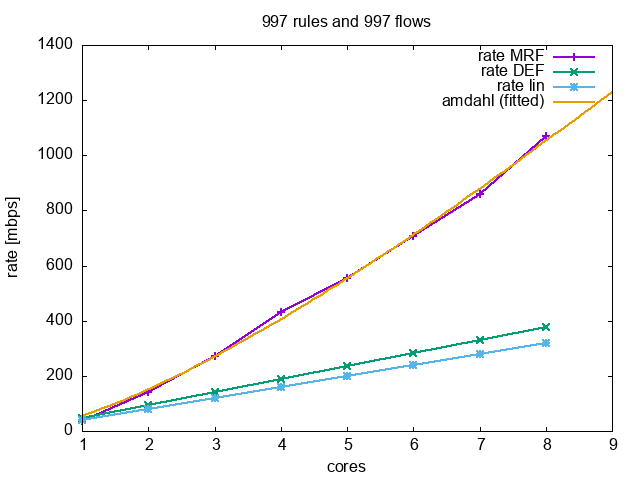
\includegraphics[width=.9\linewidth]{plot-997rules-997flows.png}
\end{center}

$$Delta_i=\frac{rate_i}{\frac{i}{i-1}rate_{i-1}}$$

\begin{center}
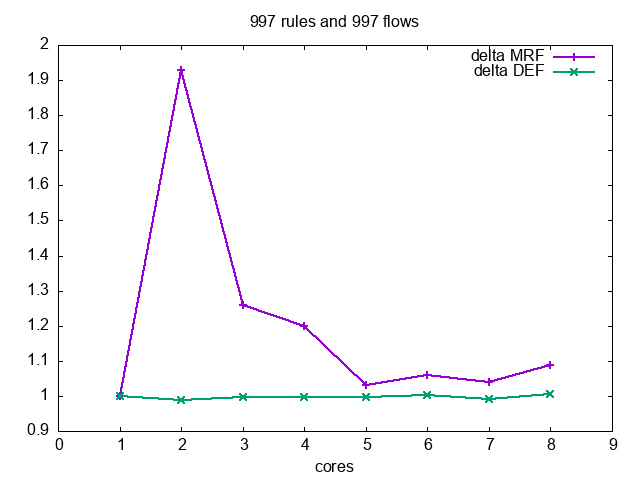
\includegraphics[width=.9\linewidth]{plot-997rules-997flows-delta.png}
\end{center}


$$prop_i=\frac{rate_i}{rate_1}$$

\begin{center}
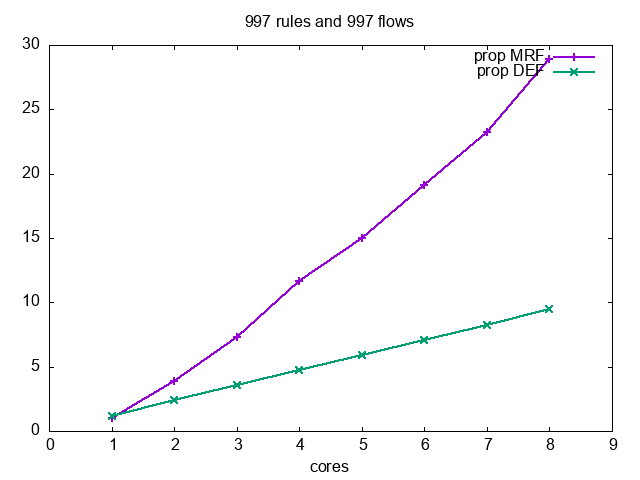
\includegraphics[width=.9\linewidth]{plot-997rules-997flows-prop.png}
\end{center}


\section*{TODOs}
\label{sec:orge85f8e6}
paper todos:
\begin{itemize}
\item setup TIPSY
\begin{itemize}
\item use classbench integration
\end{itemize}
\item load-balancer? (depends on classbench)
\item prepare two kernels:
\begin{itemize}
\item debug: lock tracing, SAL\textsubscript{DEBUG}, etc.
\item performance: current kernel
\end{itemize}
\item evaluation
\begin{itemize}
\item realistic traffic:
\begin{itemize}
\item classbench flows
\end{itemize}
\item artificial traffic:
\begin{itemize}
\item diff configs:
\begin{itemize}
\item \#nft rules,
\item \#flows,
\item \#controlled flows -> rule duplication
\end{itemize}
\item 1 cpu multiple queues?
\end{itemize}
\end{itemize}
\end{itemize}
\end{document}
